\chapter{Appendix}
\label{cha:Appendix}

% z.B. Pseudocode


\begin{figure}
    \centering
    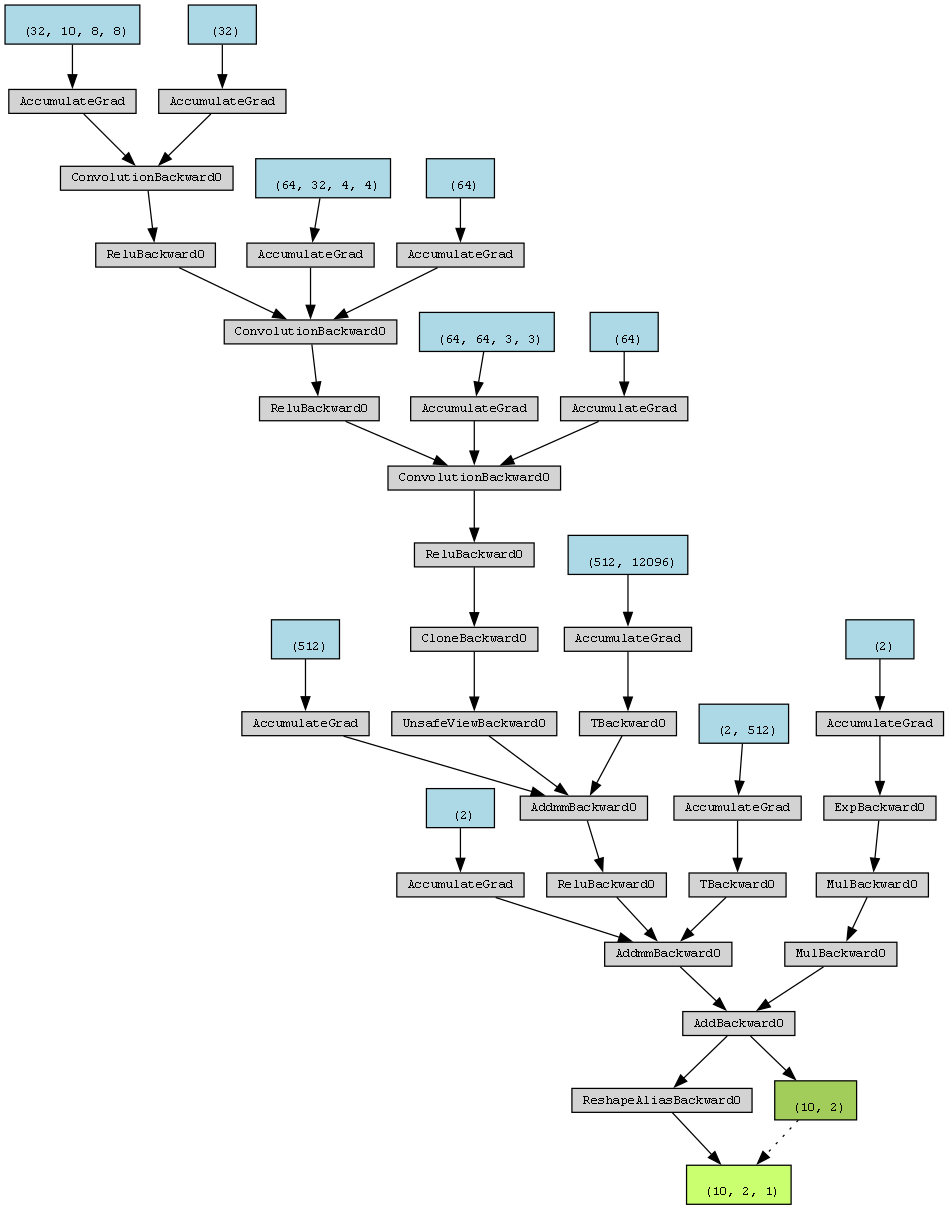
\includegraphics[width=0.5\textwidth]{Bilder/action_graph.png}
    \caption{Neural Network Architecture Action Head}
    \label{fig:action_graph}
\end{figure}

\begin{figure}
    \centering
    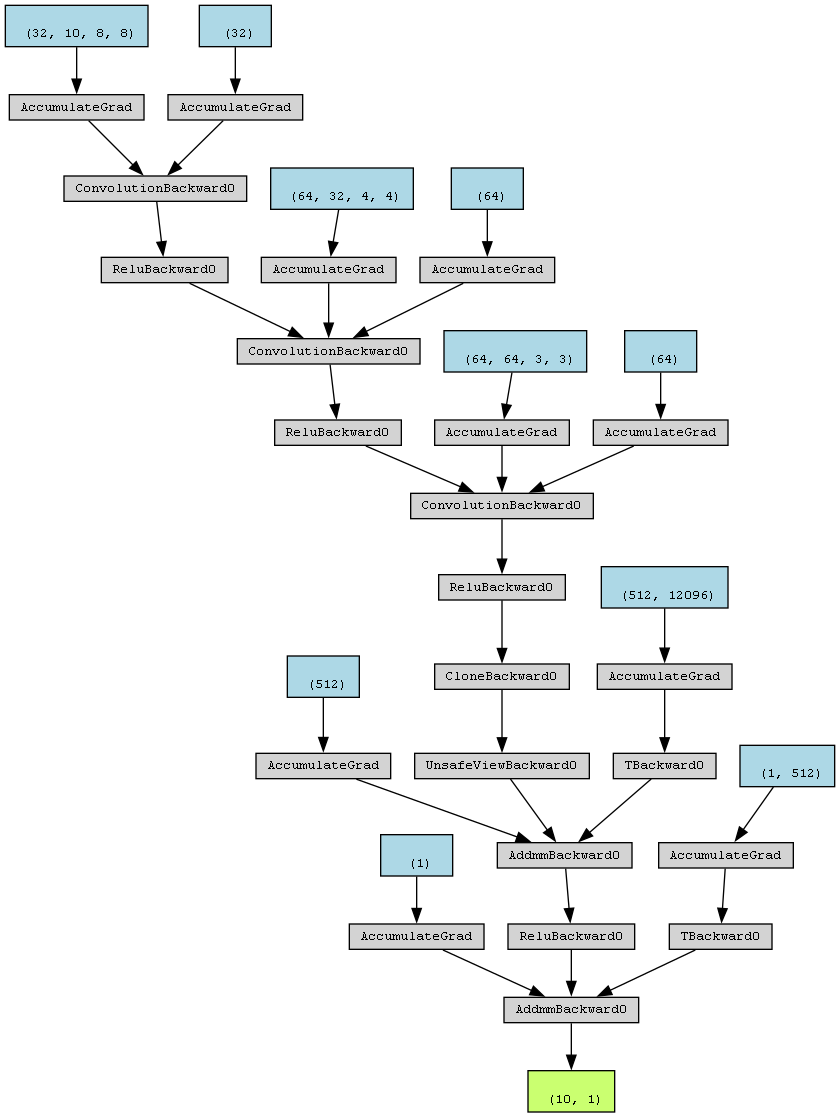
\includegraphics[width=0.5\textwidth]{Bilder/value_graph.png}
    \caption{Neural Network Architecture Value Head}
    \label{fig:value_graph}
\end{figure}

\renewcommand{\thepseudonum}{\roman{pseudonum}}
\begin{pseudocode}{Generate Map and Rotation Combinations}{ }

\PROCEDURE{generate\_map\_and\_rotations}{difficulty, n\_eval\_episodes, env}

rotationMode \GETS env.\CALL{getSpawnMode}{}\\
rotation\_range\_min, rotation\_range\_max \GETS Spawn.\CALL{getRotationRange}{rotationMode}\\

range\_width \GETS rotation\_range\_max - rotation\_range\_min\\
rotations \GETS []\\

\IF n\_eval\_episodes == 1 \THEN
    rotations.\CALL{append}{(rotation\_range\_min + range\_width)/2}\\
\ELSE
\BEGIN
    step \GETS range\_width / (n\_eval\_episodes -1)\\
    \FOR i \GETS 0 \TO n\_eval\_episodes - 1 \DO
        \BEGIN
        rotations.\CALL{append}{rotation\_range\_min + i * step}\\
        \END\\
\END\\

track\_numbers \GETS MapType.\CALL{getAllTracknumbersOfDifficulty}{difficulty}\\
tracks \GETS []\\
\FOR i \GETS 0 \TO n\_eval\_episodes - 1 \DO
\BEGIN
tracks.\CALL{append}{i \mod \CALL{len}{track\_numbers}}\\
\END\\

combinations \GETS []\\
\FOR i \GETS 0 \TO n\_eval\_episodes - 1 \DO
\BEGIN
combinations.\CALL{append}{(tracks[i], rotations[i])}\\
\END\\

\RETURN{combinations}
\ENDPROCEDURE
\label{fig:generate_track_rotation}
\end{pseudocode}





\renewcommand{\thepseudonum}{\roman{pseudonum}}
\begin{pseudocode}{Record Episode}{ }
\COMMENT{Record episode}\\

\PROCEDURE{record\_episode}{policy, env, directory}

env.\CALL{RESET}{}\\

sampled\_actions \GETS [] \\
infer\_obsstrings \GETS [] \\
step\_obsstrings \GETS [] \\

done \GETS \FALSE\\

\WHILE ! done \DO
\BEGIN
obs, obsstring \GETS env.\CALL{GetObservation}{}\\
action \GETS policy.\CALL{Infer}{obs}\\

step\_obsstring, done \GETS env.\CALL{step}{action}\\

infer\_obsstrings.\CALL{append}{obsstring}\\
step\_obsstrings.\CALL{append}{step\_obsstring}\\
sampled\_actions.\CALL{append}{action}\\
\END\\

\FOR i \GETS 0 \TO len(step\_obsstrings) \DO
    \CALL{SaveToFile}{step\_obsstrings[i], directory + ''/step\_image'' + i + ''.png''}\\
\FOR i \GETS 0 \TO len(infer\_obsstrings) \DO
    \CALL{SaveToFile}{infer\_obsstrings[i], directory + ''/infer\_image'' + i + ''.png''}\\
\FOR i \GETS 0 \TO len(sampled\_actions) \DO
    \CALL{SaveToFile}{sampled\_actions[i], directory + ''/sampled\_action'' + i + ''.npy''}\\


\ENDPROCEDURE
\label{pseudocode:record_episode}
\end{pseudocode}

\renewcommand{\thepseudonum}{\roman{pseudonum}}
\begin{pseudocode}{Replay Episode}{ }
\COMMENT{Replay episode and record processing + inference time}\\

\PROCEDURE{replay\_episode}{ policy, env, directory}

recorded\_episode\_length \GETS \CALL{LoadRecordedEpisodeLength}{directory}\\
recorded\_actions \GETS \CALL{LoadRecordedActions}{directory}\\
infer\_obs\_unity\_images \GETS \CALL{LoadInferImages}{directory}\\
step\_obs\_unity\_images \GETS \CALL{LoadStepImages}{directory}\\

reproduce\_times \GETS [] \\

replay\_time\_start \GETS \CALL{TIME}{}\\

\FOR i \GETS 0 \TO recorded\_episode\_length \DO
\BEGIN
obs \GETS \CALL{ProcessImage}{env, infer\_obs\_unity\_images[i]}\\
action \GETS policy.\CALL{Infer}{obs}\\
reproduce\_times.\CALL{append}{\CALL{TIME}{} - replay\_time\_start}\\

\CALL{AssertEqual}{action, recorded\_actions[i]}\\

replay\_time\_start \GETS \CALL{TIME}{}\\

\CALL{ProcessImage}{env, step\_obs\_unity\_images[i]}\\
\END\\
\RETURN{reproduce\_times}
\ENDPROCEDURE

\label{pseudocode:replay_episode}
\end{pseudocode}